\section{Introduction}
Maintenance scheduling is part of a class of operational problems that have proven hard to solve in practice as they
are usually modelled as resource-constrained project scheduling problems, knapsack formulations, machine scheduling problems, etc. (NP-hard~\citep{garey1979computers}).
Furthermore, for optimization to be useful in dynamic and uncertain environments where maintenance scheduling
is performed it requires tight integration into existing IT infrastructure to allow the tacit knowledge of decision makers to easily influence
the planning process. Often a number of different decision makers at different company levels take part in the
planning process. In this way the industry usually assigns responsibility for decision-making to an individual
representing only a small part of the complete process. These multiple smaller planning processes are often difficult
to map to a single mathematical model describing the whole system as elaborated by~\citep{barthelemy2002human}. Solving
operation research problems that are operational in nature have additional requirements over more typical static
problems: they have to be responsive to changing parameters; able to be assimilated into the decision-makers workflow;
allow for integration with dynamic data sources such as databases and APIs~\citep{meignan_review_2015}. Operational
aspects of operation research, as opposed to higher level strategic and tactical ones, are characterized by extensive
amounts coordination and negotiation on proposed schedules often in a short amount of time~\citep{palmerMaintenancePlanningScheduling2019}.

The lack of integration into the schedulers and supervisors workflow and lack of responsiveness can lead to a situation
where solutions are not directly implemented in practice but instead only provides initial suggestions~\citep{meignan_review_2015}.
Theses initial suggestions are then iterated on elsewhere in the scheduling process usually through much more manual means.
In~\citep{barthelemy2002human} the authors argue that many problems that operation research aim to solve are often composed
of a group of individuals whose decisions are consolidated into an "epistemic subject" for which a mathematical model can be formulated
and solved, with many scheduling problems being good examples. However, often multiple actors have different
views on what constitutes an optimal schedule hence resulting in multiple-objectives. Even if multi-objective
optimization~\citep{ehrgott2002multiple} is applied to find a Pareto Front~\citep{Pareto1897} a negotiating process
still is needed between the actors to select the final schedule.

This paper proposes a solution method that will allow for real-time optimization
based on actor/user interaction and a connection to a dynamic data source,
effectively managing the changes to the parameter space as they occur. The proposed solution
method will be tested on the weekly maintenance scheduling problem \citet{palmerMaintenancePlanningScheduling2019}
which closely resembles a variant of the multi-compartment multi-knapsack problem (MCMKP)~\cite{do2007constrained}. It
should be noted that the scientific maintenance scheduling literature can deviate
significantly from its practical implementation which is also detailed in
\citep{palmerMaintenancePlanningScheduling2019}. The solution method is
based on the large neighborhood search (LNS~\cite{shaw1998using}) metaheuristic and is in this
paper describes as actor-based large neighborhood search (AbLNS). LNS
was chosen due to its properties of naturally being able to work with and fix
infeasible solutions and because of its state of the art performance on various scheduling
problems \citep{gendreauHandbookMetaheuristics2019}.

To understand the need for actor-based methods some
background knowledge will be required about the maintenance scheduling process.
Figure~\ref{fig:integrated:maintenance-process} illustrates the general setup
of a maintenance planning and scheduling system. The system's actors
have the following responsibilities: the planner generates the work orders that
are to be scheduled; each scheduler creates weekly schedules for a set of work orders ; 
based on the weekly schedule the supervisors assign work order
activities to technicians; the
technicians executes the work in sequential pattern. Each planning problem is matched 
by a corresponding optimization problem, for the scheduler, it is a variation of the
multi-compartment multi-knapsack problem, for the supervisor it is a variation of the 
assignment problem and for the technicians it is a single machine scheduling problem.

The idea of ownership of a work order is crucial to understand the necessity of
actor-based approaches. Throughout the scheduling process a
work order is always owned by a specific actor and he alone is allow to modify/execute it. This
means that a single model approach is very difficult to implement in practice
as a work order is modelled differently depending on the actor that currently
owns it. This highlights another point in maintenance scheduling: that
the stochastic nature of the maintenance scheduling process can be handled using
a change of model, each with different levels of aggregation and different sets
of constraints, opposed to more academic approaches such as fuzzy logic and
stochastic optimization. When the inherrent uncertainties manifest themselves
during planning or execution, work orders are rescheduled by moving between
the different actors, meaning that the stochastic elements of maintenance
scheduling are handled by \textbf{dynamic rescheduling between the actors}.

\begin{figure}
	\usetikzlibrary{positioning}
\definecolor{red}{HTML}{8A3F3A}
\definecolor{yellow}{HTML}{E0BB3C}
\definecolor{blue}{HTML}{4569E0}
\definecolor{green}{HTML}{17E561}
\definecolor{other}{HTML}{6A939E}

% DTU Colors
\definecolor{dtu-corporate-red}{HTML}{990000}
\definecolor{dtu-white}{HTML}{ffffff}
\definecolor{dtu-black}{HTML}{000000}
\definecolor{dtu-blue}{HTML}{2F3EEA}
\definecolor{dtu-bright-green}{HTML}{1FD082}
\definecolor{dtu-navy-blue}{HTML}{030F4F}
\definecolor{dtu-yellow}{HTML}{F6D04D}
\definecolor{dtu-orange}{HTML}{FC7634}
\definecolor{dtu-pink}{HTML}{F7BBB1}
\definecolor{dtu-grey}{HTML}{DADADA}
\definecolor{dtu-red}{HTML}{E83F48}
\definecolor{dtu-green}{HTML}{008835}
\definecolor{dtu-purple}{HTML}{79238E}


\newlength{\basisa}
\setlength{\basisa}{1cm}
\centering
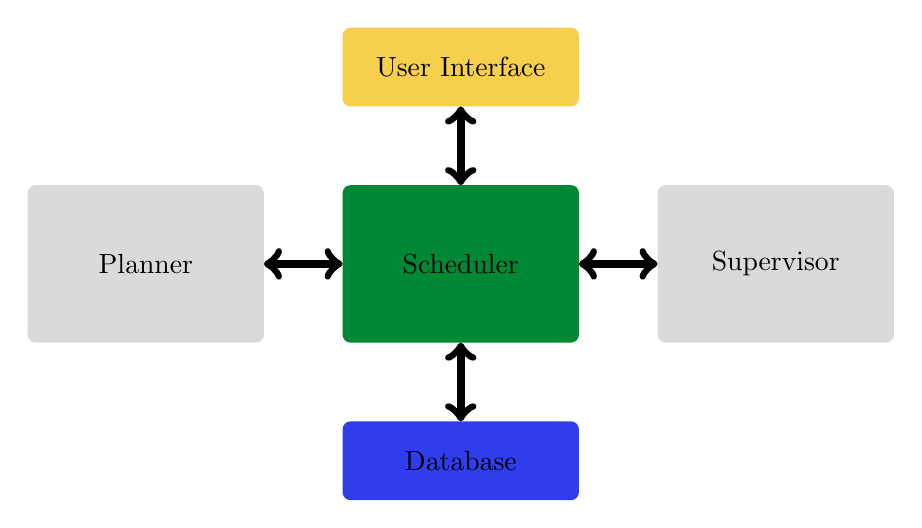
\begin{tikzpicture}[line width=0.0\basisa]
    \draw (4.0\basisa,4.0\basisa) 
		node[minimum height=2\basisa,fill=dtu-grey,minimum width=3\basisa,rounded corners=0.1\basisa] 
			(Planner) {Planner};
    \draw (12.0\basisa,4.0\basisa) 
		node[minimum height=2\basisa,fill=dtu-grey,minimum width=3\basisa,rounded corners=0.1\basisa] 
			(Supervisor) {Supervisor};

			
    \draw (8.0\basisa,4.0\basisa) 
		node[minimum height=2\basisa,fill=dtu-green,minimum width=3\basisa,rounded corners=0.1\basisa] 
			(Scheduler) {Scheduler};
	
    \draw (8.0\basisa,1.5\basisa) 
		node[minimum height=1\basisa,fill=dtu-blue,minimum width=3\basisa,rounded corners=0.1\basisa] 
			(Database) {Database};

    \draw (8.0\basisa,6.5\basisa) 
		node[minimum height=1\basisa,fill=dtu-yellow,minimum width=3\basisa,rounded corners=0.1\basisa] 
			(UserInterface) {User Interface};

	\draw[<->, thick, line width=0.1\basisa] (Planner) -- (Scheduler);
	\draw[<->, thick, line width=0.1\basisa] (Scheduler) -- (Supervisor);
	\draw[<->, thick, line width=0.1\basisa] (Scheduler) -- (Database);
	\draw[<->, thick, line width=0.1\basisa] (Scheduler) -- (UserInterface);
\end{tikzpicture}

	\caption{Simple overview of the scheduling process with its primary types of actors. The planner, the scheduler, the supervisor(s), and the technicians.
		The green color highlights the scheduler as it the actor in the maintenance scheduling process that is the foundation for the paper.}
	\label{fig:integrated:maintenance-process}
\end{figure}

The main contribution of this article is to provide a
modular scalable optimization component,  based on a proven
metaheuristic to support a business process composed from
smaller mathematical  models in a framework, instead of a
larger integrated mathematical model.

The paper is divided into four different sections. Section \ref{sec:2-solution-method} explains
the weekly maintenance scheduling model in detail and forms the foundation of the paper. 
Section \ref{sec:3-results} shows the results that come from the metaheuristic implemented,
where it will be affected by the simulated user interaction. Section \ref{sec:4-discussion} 
will discuss the implications of the research and estabslish a future research direction.
All source code for the implemented system can be found at \citep{scipo-code-ordinator_api},
instance data is confidential and cannot be shared publicly.

\subsection{The Weekly (Period) Maintenance Scheduling Model}
The weekly maintenance scheduling model for the problem
is a variant of the  Multi-compartment Multi-knapsack Problem with capacity penalties MCMKP.
The notation used to describe the dynamical aspects in the model is based on the notation
from the dynamic metaheuristics literature as found in \cite{yangMetaheuristicsDynamicCombinatorial2013}.
Here the $\VarMetaTime$ is added as a time variable on all sets, parameters, and variables that are
subject to change while the metaheuristic is running. This enables us to be precise in the timing on
the messages that are send to the Ab-LNS and understand how it reacts in real-time.
A company performing maintenance usually creates weekly maintenance plans for
the next $\ElementPeriod \in \SetPeriod$ period. The weekly schedule is created
centrally and consists of scheduling the $\ElementWorkOrder \in \SetWorkOrder$
work orders, i.e. maintenance tasks, such that all $\ElementWorkOrder$
are scheduled into a specific period $\ElementPeriod$. Each work order $
\ElementWorkOrder$ requires some resources $\ElementResource \in \SetResource$
to be carried out, e.g. man-power with different qualifications. Each of these
resources are available in limited amounts given by $\ParStrategicResource$. To correct
for possible manual interventions that can make the problem infeasible a penalty (
$\ParStrategicResourcePenalty$) is introduced. The urgency of the different maintenance work order ($\ElementWorkOrder$)
varies and is reflected in a "tardiness" for carrying out a maintenance work
order in a certain period given by $\ParStrategicUrgency$. The $\ParStrategicUrgency$ also
captures the tardiness of the individual work orders ($\ElementWorkOrder$), meaning that
the value gained from scheduling work orders late is decreasing. Urgent tasks have
decreasing value the further out the period $\ElementPeriod$ becomes.
Furthermore, two sets exists which will either require work order $\ElementWorkOrder$ to be carried
out in period $\ElementPeriod$ or not carried out in a period $\ElementPeriod$.
These sets are $(\ElementWorkOrder,\ElementPeriod) \in
\ParStrategicInclude$ for inclusion and  $(\ElementWorkOrder, \ElementPeriod) \in
\ParStrategicExclude$ for exclusion.


\newpage
\begin{alignat}{2}
	& \text{\rule{\linewidth}{0.4pt}} \notag\\
	& \textbf{Meta variables:} \notag\\
	& \ElementScheduler \in \SetScheduler \\
	& \VarTacticalWork{}{} \\ 
	& \tau \in [0, \infty] \\
	& \text{\rule{\linewidth}{0.4pt}} \notag\\
	& \textbf{Minimize:} \notag                                                                                                                                                        \\
	& \sum_{\ElementWorkOrder \in \SetWorkOrder{}} \sum_{\ElementPeriod \in \SetPeriod} \ParStrategicValue \cdot \VarStrategicWorkOrderAssignment{\ElementWorkOrder}{\ElementPeriod}  \notag\\ 
	& + \sum_{\ElementPeriod \in \SetPeriod} \sum_{\ElementResource \in \SetResource} \ParStrategicPenalty \cdot \VarStrategicExcess     \notag                                              \\
	& + \sum_{\ElementPeriod \in \SetPeriod} \sum_{\ElementWorkOrder1 \in \SetWorkOrder{}} \sum_{\ElementWorkOrder2 \in \SetWorkOrder{}} 	 \quad \ParClusteringValue \cdot \VarStrategicWorkOrderAssignment{\ElementWorkOrder1}{\ElementPeriod} \cdot \VarStrategicWorkOrderAssignment{\ElementWorkOrder2}{\ElementPeriod}  \\
	& \text{\rule{\linewidth}{0.4pt}} \notag\\
	& \textbf{Subject to:} \notag                                                                                                                                                      \\
	& \sum_{\ElementWorkOrder \in \SetWorkOrder{}} \ParStrategicWorkOrderWeight \cdot \VarStrategicWorkOrderAssignment{\ElementWorkOrder}{\ElementPeriod} \leq \ \ParStrategicResource + \VarStrategicExcess                                                                           \quad \forall \ElementPeriod \in \SetPeriod \quad \forall \ElementResource \in \SetResource                                                                                      \\
	& \sum_{\ElementWorkOrder \in \SetWorkOrder{}} \VarStrategicWorkOrderAssignment{\ElementWorkOrder}{\ElementPeriod} = 1              \quad \forall \ElementPeriod \in \SetPeriod                                                                                                                                      \\
	& \VarStrategicWorkOrderAssignment{\ElementWorkOrder}{\ElementPeriod} = 0                                                            \quad \forall (\ElementWorkOrder, \ElementPeriod) \in \ParStrategicExclude                                                                                                       \\
	& \VarStrategicWorkOrderAssignment{\ElementWorkOrder}{\ElementPeriod} = 1                                                            \quad \forall (\ElementWorkOrder, \ElementPeriod) \in \ParStrategicInclude                                                                                                       \\
	& \VarStrategicWorkOrderAssignment{\ElementWorkOrder}{\ElementPeriod} \in \{0, 1\}                                                   \quad \forall \ElementWorkOrder \in \SetWorkOrder{} \quad \forall \ElementPeriod \in \SetPeriod                                                                                 \\ 
	& \VarStrategicExcess \in \mathbb{R}^{+}                                                                                             \quad \forall \ElementPeriod \in \SetPeriod \quad \forall \ElementResource \in \SetResource                                                                                  \\ 
	& \text{\rule{\linewidth}{0.4pt}} \notag
\end{alignat}
\newpage


\strategicmodel[clustering=true, beta=false]

The meta variables defines the broader setting that the model in implemented in.
Equation~\eqref{eqn:meta:scheduler:strategic} specicies that the model is
implemented for scheduler \ElementScheduler. 
Equation~\eqref{eqn:meta:time:strategic} is the time variable that binds the whole
system together.

The objective function~\eqref{eqn:objective:strategic},  maximizes the total
weighted assignment of all work order subtractied by the penalty $\ParStrategicResourcePenalty$
for exceeding the resource capacity given in equation
\eqref{eqn:strategic:constraint:resource}. The third term of the objective
function handles the $\ParClusteringValue$ which turns the model into a quadratic
problem. This term optimizes the value of putting two work orders in the same
period, if they have share similarity like close proximity, same piece of equipment
, etc.  Equation \eqref{eqn:strategic:constraint:resource} ensures
that all the $\ParOperationWork{wr}$ for each activity in a work
order, given that it has been assigned, is lower than the $\ParStrategicResource$ for each
$\ElementPeriod$ and for each resources $\ElementResource$. $\ParStrategicResourcePenalty$ is the
amount of exceeded capacity that is needed for the current assignment of work
order to be feasible. Equation \eqref{eqn:constraint:strategic:schedule_once}
makes sure that each work order is assigned to at least a one
period. Equation \eqref{eqn:strategic:constraint:exclude}
excludes a work order from a certain period and equation
\eqref{eqn:constraint:strategic:include} forces a specific work order to be
included in a specific period. Constraint \eqref{eqn:variable:strategic:assignment}
and \eqref{eqn:variable:strateigc:penalty} specify the variable domain
for $\VarStrategicWorkOrderAssignment{\ElementWorkOrder}{\ElementPeriod}$
and $\ParStrategicResourcePenalty$ respectively. The effects of changing $
\ParStrategicInclude$, $\ParStrategicExclude$, $\ParStrategicResource$, and $
\ParStrategicUrgency$ in real-time will be examined in the results section~\ref{sec:3-results} to
determine their effects on the weekly schedules and the objective value.
